\chapter{Threefold Data}

\renewcommand{\thefootnote}{\fnsymbol{footnote}} 
\setcounter{footnote}{0}

\begin{tabular}{llll}
\toprule
\textbf{Name:} & 4.8 \hspace{0.3\textwidth} & \textbf{Description:} & Blow up of $Q$ in a line\\
\midrule
\end{tabular}

\begin{figure}[h]
\centering


\label{fig:data230b}
\resizebox{0.9\linewidth}{!}{
\begin{subfigure}[b]{0.30\textwidth}
\centering
  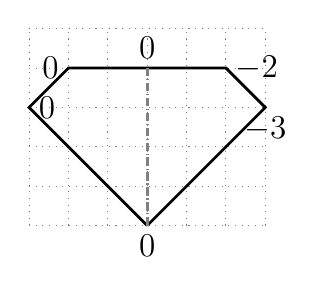
\begin{tikzpicture}[scale=0.5]
   	 \draw[dotted,step=1,gray,] (-3,-3) grid (3,2); \draw[line width = 1pt] (0,-3) --
     (-3,0) -- (-2,1)--(2,1)--
 	 (3,0)--(0,-3); \draw[densely dashdotted, gray, line width = 1.2pt] (0,-3) -- (0,1);
 	 \node at (0,-3) [below] {\large{$0$}};
 	 \node at (-3,0) [right] {\large{$0$}};
 	 \node at (-2,1) [left] {\large{$0$}};
 	 \node at (2,1) [right] {\large{$-2$}};
 	 \node at (3,0) [below] {\large{$-3$}};
 	 \node at (0,1) [above] {\large{$0$}};
	\end{tikzpicture}
	\caption*{$\Phi_0$}
\end{subfigure}
\begin{subfigure}[b]{0.30\textwidth}
	\centering
 	 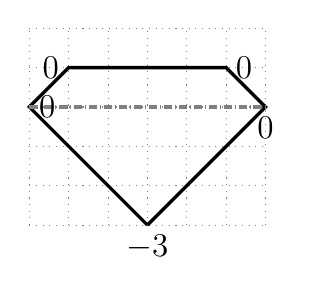
\begin{tikzpicture}[scale=0.5]
 	   \draw[dotted,step=1,gray] (-3,-3) grid (3,2); \draw[line width = 1.2pt] (0,-3) --
 	   (-3,0) -- (-2,1)--(2,1)--
 	   (3,0)--(0,-3); \draw[densely dashdotted, gray,line width = 1.2pt] (-3,0) -- (3,0);
 	 \node at (0,-3) [below] {\large{$-3$}};
 	 \node at (-3,0) [right] {\large{$0$}};
 	 \node at (-2,1) [left] {\large{$0$}};
 	 \node at (2,1) [right] {\large{$0$}};
 	 \node at (3,0) [below] {\large{$0$}};
	\end{tikzpicture}
	\caption*{$\Phi_1$}
\end{subfigure}
\begin{subfigure}[b]{0.30\textwidth}
	\centering
 	 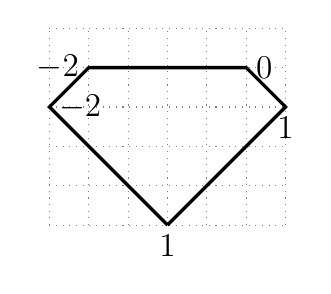
\begin{tikzpicture}[scale=0.5]
 	   \draw[dotted,step=1,gray] (-3,-3) grid (3,2); \draw[line width = 1.2pt] (0,-3) --
 	   (-3,0) -- (-2,1)--(2,1)--
 	   (3,0)--(0,-3);
 	 \node at (0,-3) [below] {\large{$1$}};
 	 \node at (-3,0) [right] {\large{$-2$}};
 	 \node at (-2,1) [left] {\large{$-2$}};
 	 \node at (2,1) [right] {\large{$0$}};
 	 \node at (3,0) [below] {\large{$1$}};
	\end{tikzpicture}
	\caption*{$\Phi_\infty$}
\end{subfigure}
\begin{subfigure}[b]{0.40\textwidth}
	\centering
 	 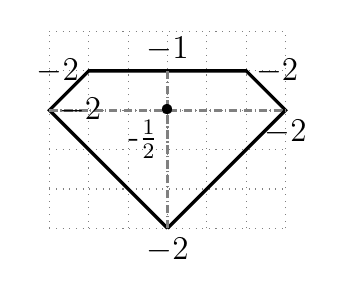
\begin{tikzpicture}[scale=0.5]
 	   \draw[dotted,step=1,gray] (-3,-3) grid (3,2); \draw[line width = 1.2pt] (0,-3) --
 	   (-3,0) -- (-2,1)--(2,1)--
 	   (3,0)--(0,-3); \draw[densely dashdotted, gray,line width = 1.2pt] (-3,0) -- (3,0); \draw[densely dashdotted, gray,line width = 1.2pt] (0,-3) -- (0,1) ;
 	 \node at (0,-3) [below] {\large{$-2$}};
 	 \node at (-3,0) [right] {\large{$-2$}};
 	 \node at (-2,1) [left] {\large{$-2$}};
 	 \node at (2,1) [right] {\large{$-2$}};
 	 \node at (3,0) [below] {\large{$-2$}};
 	 \node at (0,0) [below left] {\large{-$\frac{1}{2}$}};
 	 \node at (0,1) [above] {\large{$-1$}};
 	 \draw (0,0) node {\textbullet};
	\end{tikzpicture}
	\caption*{$\deg \Phi $}
\end{subfigure}
}
\end{figure}


\begin{tabular}{llll}
\toprule
\textbf{Name:} & 2.31 \hspace{0.3\textwidth} & \textbf{Description:} & Blow up of $Q$ in a line \\
{$\sigma$:} & \ & \ & \ \\
\midrule
\end{tabular}

\begin{figure}[h]
\centering
\label{fig:data231}
\resizebox{0.9\linewidth}{!}{
\begin{subfigure}[b]{0.30\textwidth}
\centering
  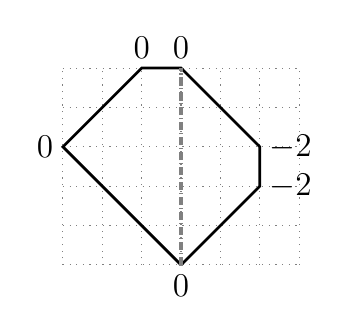
\begin{tikzpicture}[scale=0.5]
   	 \draw[dotted,step=1,gray,] (-3,-3) grid (3,2); \draw[line width = 1pt] (0,-3) --
     (-3,0) -- (-1,2)--(0,2)--
 	 (2,0)--(2,-1) -- (0,-3); \draw[densely dashdotted, gray, line width = 1.2pt] (0,-3) -- (0,2);
 	 \node at (0,-3) [below] {\large{$0$}};
 	 \node at (-3,0) [left] {\large{$0$}};
 	 \node at (-1,2) [above] {\large{$0$}};
 	 \node at (0,2) [above] {\large{$0$}};
 	 \node at (2,0) [right] {\large{$-2$}};
 	 \node at (2,-1) [right] {\large{$-2$}};
	\end{tikzpicture}
	\caption*{$\Phi_0$}
\end{subfigure}
\begin{subfigure}[b]{0.30\textwidth}
	\centering
 	 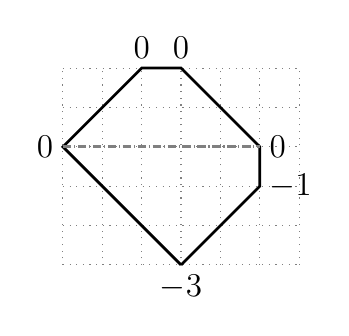
\begin{tikzpicture}[scale=0.5]
 	   \draw[dotted,step=1,gray] (-3,-3) grid (3,2); \draw[line width = 1pt] (0,-3) --
     (-3,0) -- (-1,2)--(0,2)--
 	 (2,0)--(2,-1) -- (0,-3); \draw[densely dashdotted, gray,line width = 1.2pt] (-3,0) -- (2,0);
 	 \node at (0,-3) [below] {\large{$-3$}};
 	 \node at (-3,0) [left] {\large{$0$}};
 	 \node at (-1,2) [above] {\large{$0$}};
 	 \node at (0,2) [above] {\large{$0$}};
 	 \node at (2,0) [right] {\large{$0$}};
 	 \node at (2,-1) [right] {\large{$-1$}};
	\end{tikzpicture}
	\caption*{$\Phi_1$}
\end{subfigure}
\begin{subfigure}[b]{0.30\textwidth}
	\centering
 	 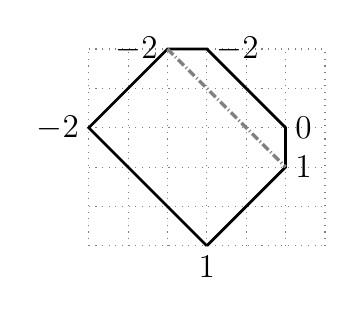
\begin{tikzpicture}[scale=0.5]
 	   \draw[dotted,step=1,gray] (-3,-3) grid (3,2); \draw[line width = 1pt] (0,-3) --
     (-3,0) -- (-1,2)--(0,2)--
 	 (2,0)--(2,-1) -- (0,-3); \draw[densely dashdotted, gray,line width = 1.2pt] (-1,2) -- (2,-1);
 	 \node at (0,-3) [below] {\large{$1$}};
 	 \node at (-3,0) [left] {\large{$-2$}};
 	 \node at (-1,2) [left] {\large{$-2$}};
 	 \node at (0,2) [right] {\large{$-2$}};
 	 \node at (2,0) [right] {\large{$0$}};
 	 \node at (2,-1) [right] {\large{$1$}};
	\end{tikzpicture}
	\caption*{$\Phi_\infty$}
\end{subfigure}
\begin{subfigure}[b]{0.40\textwidth}
	\centering
 	 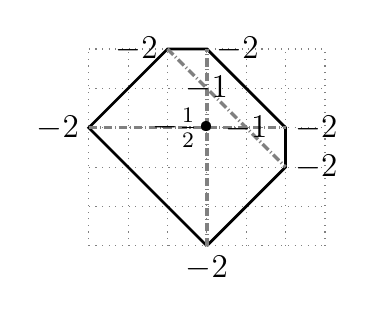
\begin{tikzpicture}[scale=0.5]
 	   \draw[dotted,step=1,gray] (-3,-3) grid (3,2); \draw[line width = 1pt] (0,-3) --
     (-3,0) -- (-1,2)--(0,2)--
 	 (2,0)--(2,-1) -- (0,-3); \draw[densely dashdotted, gray, line width = 1.2pt] (0,-3) -- (0,2);  \draw[densely dashdotted, gray,line width = 1.2pt] (-3,0) -- (2,0); \draw[densely dashdotted, gray,line width = 1.2pt] (-1,2) -- (2,-1);
 	 \node at (0,-3) [below] {\large{$-2$}};
 	 \node at (-3,0) [left] {\large{$-2$}};
 	 \node at (-1,2) [left] {\large{$-2$}};
 	 \node at (0,2) [right] {\large{$-2$}};
 	 \node at (2,0) [right] {\large{$-2$}};
 	 \node at (2,-1) [right] {\large{$-2$}};
 	 \node at (1,0) {\large{$-1$}};
 	 \node at (0,1) {\large{$-1$}};
 	 \node at (0,0) [left] {\large{$-\frac{1}{2}$}};
 	 \draw (0,0) node {\textbullet};
	\end{tikzpicture}
	\caption*{$\deg \Phi $}
\end{subfigure}
}
\end{figure}

\begin{align*}
g(\xi) &= \frac{1}{\xi_{2}^{4}}\cdot\left({\left(2 \, \xi_{2}^{3} - 3 \, \xi_{2} - 3\right)} e^{\left(4 \, \xi_{2}\right)} + 12 \, \xi_{2} e^{\left(3 \, \xi_{2}\right)} + 3 \, \xi_{2} + 3\right) e^{\left(-3 \, \xi_{2}\right)} \\
h_0(\xi_2) &= \frac{1}{3\xi_2^{4}}\cdot
{\left({\left(2   \xi_2^{3} - 3   \xi_2 - 3\right)} e^{4   \xi_2} + 3   {\left(3   \xi_2^{2} + 2\right)} e^{3   \xi_2} - 3   \xi_2 - 3\right)} e^{-3   \xi_2}
\\
h_1(\xi_2) &= \frac{1}{6   \xi_2^{4}}\cdot
{\left({\left(8   \xi_2^{3} + 6   \xi_2^{2} - 3\right)} e^{4   \xi_2} - 12   {\left(3   \xi_2^{2} - 3   \xi_2 + 1\right)} e^{3   \xi_2} + 12   \xi_2 + 15\right)} e^{-3   \xi_2} \\
h_\infty(\xi_2) &= -\frac{1}{6   \xi_2^{4}}\cdot
{\left(2   {\left(2   \xi_2^{3} - 3   \xi_2 - 3\right)} e^{4   \xi_2} - 3   {\left(3   \xi_2^{2} - 12   \xi_2 + 2\right)} e^{3   \xi_2} + 12   \xi_2 + 12\right)} e^{-3   \xi_2} \\
h_y(\xi_2) &= \frac{1}{6   \xi_2^{4}}\cdot{\left({\left(8   \xi_2^{3} + 6   \xi_2^{2} - 3\right)} e^{4   \xi_2 } - 3   {\left(3   \xi_2^{2} - 2\right)} e^{3   \xi_2} - 6   y - 3\right)} e^{-3   \xi_2} 
\end{align*}
\begin{align*}
1.087 &< h_0(\xi_2) < 1.458 \\
2.178 &< h_1(\xi_2) < 2.470 \\
0.446 &< h_\infty(\xi_2) < 0.827 \\
4.151 &< h_y(\xi_2) < 4.309 \ \ \ \ \ \ \   \left( \text{for } y \not \in \{0,1,\infty\} \right)
\end{align*}

\begin{tabular}{llll}
\toprule
\textbf{Name:} & 3.8* \hspace{0.3\textwidth} & \textbf{Description:} & Blow up of $Q$ in a line\\
\midrule
\end{tabular}

\begin{figure}[h]
\centering
\label{fig:data38*}
\resizebox{0.9\linewidth}{!}{
\begin{subfigure}[b]{0.30\textwidth}
\centering
  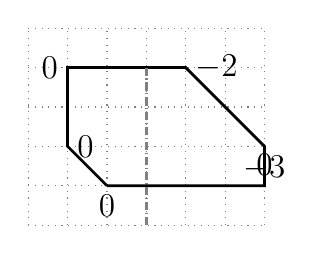
\begin{tikzpicture}[scale=0.5]
   	 \draw[dotted,step=1,gray,] (-3,-3) grid (3,2); \draw[line width = 1pt] (-1,-2) --
     (-2,-1) -- (-2,1)--(1,1)--
 	 (3,-1)--(3,-2) -- (-1,-2); \draw[densely dashdotted, gray, line width = 1.2pt] (0,-3) -- (0,1);
 	 \node at (-1,-2) [below] {\large{$0$}};
 	 \node at (-2,-1) [right] {\large{$0$}};
 	 \node at (-2,1) [left] {\large{$0$}};
 	 \node at (1,1) [right] {\large{$-2$}};
 	 \node at (3,-1) [below] {\large{$-3$}};
 	 \node at (3,-2) [above] {\large{$0$}};
	\end{tikzpicture}
	\caption*{$\Phi_0$}
\end{subfigure}
\begin{subfigure}[b]{0.30\textwidth}
	\centering
 	 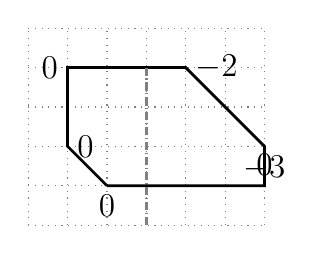
\begin{tikzpicture}[scale=0.5]
   	 \draw[dotted,step=1,gray,] (-3,-3) grid (3,2); \draw[line width = 1pt] (-1,-2) --
     (-2,-1) -- (-2,1)--(1,1)-- (3,-1)--(3,-2) -- (-1,-2); \draw[densely dashdotted, gray, line width = 1.2pt] (0,-3) -- (0,1);
 	 \node at (-1,-2) [below] {\large{$0$}};
 	 \node at (-2,-1) [right] {\large{$0$}};
 	 \node at (-2,1) [left] {\large{$0$}};
 	 \node at (1,1) [right] {\large{$-2$}};
 	 \node at (3,-1) [below] {\large{$-3$}};
 	 \node at (3,-2) [above] {\large{$0$}};
	\end{tikzpicture}
	\caption*{$\Phi_1$}
\end{subfigure}
\begin{subfigure}[b]{0.30\textwidth}
	\centering
 	 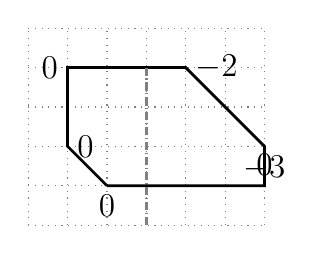
\begin{tikzpicture}[scale=0.5]
   	 \draw[dotted,step=1,gray,] (-3,-3) grid (3,2); \draw[line width = 1pt] (-1,-2) --
     (-2,-1) -- (-2,1)--(1,1)-- (3,-1)--(3,-2) -- (-1,-2); \draw[densely dashdotted, gray, line width = 1.2pt] (0,-3) -- (0,1);
 	 \node at (-1,-2) [below] {\large{$0$}};
 	 \node at (-2,-1) [right] {\large{$0$}};
 	 \node at (-2,1) [left] {\large{$0$}};
 	 \node at (1,1) [right] {\large{$-2$}};
 	 \node at (3,-1) [below] {\large{$-3$}};
 	 \node at (3,-2) [above] {\large{$0$}};
	\end{tikzpicture}
	\caption*{$\Phi_\infty$}
\end{subfigure}
\begin{subfigure}[b]{0.40\textwidth}
	\centering
 	 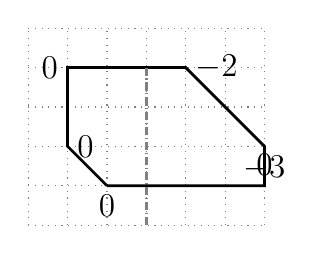
\begin{tikzpicture}[scale=0.5]
   	 \draw[dotted,step=1,gray,] (-3,-3) grid (3,2); \draw[line width = 1pt] (-1,-2) --
     (-2,-1) -- (-2,1)--(1,1)-- (3,-1)--(3,-2) -- (-1,-2); \draw[densely dashdotted, gray, line width = 1.2pt] (0,-3) -- (0,1);
 	 \node at (-1,-2) [below] {\large{$0$}};
 	 \node at (-2,-1) [right] {\large{$0$}};
 	 \node at (-2,1) [left] {\large{$0$}};
 	 \node at (1,1) [right] {\large{$-2$}};
 	 \node at (3,-1) [below] {\large{$-3$}};
 	 \node at (3,-2) [above] {\large{$0$}};
	\end{tikzpicture}
	\caption*{$\deg \Phi $}
\end{subfigure}
}
\end{figure}

\begin{align*}
g(\xi) &= \frac{1}{\xi_{2}^{4}}\cdot\left({\left(2 \, \xi_{2}^{3} - 3 \, \xi_{2} - 3\right)} e^{\left(4 \, \xi_{2}\right)} + 12 \, \xi_{2} e^{\left(3 \, \xi_{2}\right)} + 3 \, \xi_{2} + 3\right) e^{\left(-3 \, \xi_{2}\right)} \\
h_0(\xi_2) &= \frac{1}{3\xi_2^{4}}\cdot
{\left({\left(2   \xi_2^{3} - 3   \xi_2 - 3\right)} e^{4   \xi_2} + 3   {\left(3   \xi_2^{2} + 2\right)} e^{3   \xi_2} - 3   \xi_2 - 3\right)} e^{-3   \xi_2}
\\
h_1(\xi_2) &= \frac{1}{6   \xi_2^{4}}\cdot
{\left({\left(8   \xi_2^{3} + 6   \xi_2^{2} - 3\right)} e^{4   \xi_2} - 12   {\left(3   \xi_2^{2} - 3   \xi_2 + 1\right)} e^{3   \xi_2} + 12   \xi_2 + 15\right)} e^{-3   \xi_2} \\
h_\infty(\xi_2) &= -\frac{1}{6   \xi_2^{4}}\cdot
{\left(2   {\left(2   \xi_2^{3} - 3   \xi_2 - 3\right)} e^{4   \xi_2} - 3   {\left(3   \xi_2^{2} - 12   \xi_2 + 2\right)} e^{3   \xi_2} + 12   \xi_2 + 12\right)} e^{-3   \xi_2} \\
h_y(\xi_2) &= \frac{1}{6   \xi_2^{4}}\cdot{\left({\left(8   \xi_2^{3} + 6   \xi_2^{2} - 3\right)} e^{4   \xi_2 } - 3   {\left(3   \xi_2^{2} - 2\right)} e^{3   \xi_2} - 6   y - 3\right)} e^{-3   \xi_2} 
\end{align*}
\begin{align*}
1.087 &< h_0(\xi_2) < 1.458 \\
2.178 &< h_1(\xi_2) < 2.470 \\
0.446 &< h_\infty(\xi_2) < 0.827 \\
4.151 &< h_y(\xi_2) < 4.309 \ \ \ \ \ \ \   \left( \text{for } y \not \in \{0,1,\infty\} \right)
\end{align*}



\begin{tabular}{llll}
\toprule
\textbf{Name:} & 3.18 \hspace{0.3\textwidth} & \textbf{Description:} & Blow up of $Q$ in a line\\
\midrule
\end{tabular}

\begin{figure}[h]
\centering
\label{fig:data318}
\resizebox{0.9\linewidth}{!}{
\begin{subfigure}[b]{0.30\textwidth}
\centering
  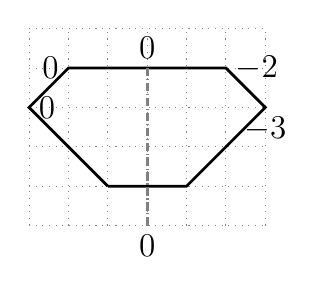
\begin{tikzpicture}[scale=0.5]
   	 \draw[dotted,step=1,gray,] (-3,-3) grid (3,2); \draw[line width = 1pt] (-1,-2) --
     (-3,0) -- (-2,1)--(2,1)--
 	 (3,0)--(1,-2) -- (-1,-2); \draw[densely dashdotted, gray, line width = 1.2pt] (0,-3) -- (0,1);
 	 \node at (0,-3) [below] {\large{$0$}};
 	 \node at (-3,0) [right] {\large{$0$}};
 	 \node at (-2,1) [left] {\large{$0$}};
 	 \node at (2,1) [right] {\large{$-2$}};
 	 \node at (3,0) [below] {\large{$-3$}};
 	 \node at (0,1) [above] {\large{$0$}};
	\end{tikzpicture}
	\caption*{$\Phi_0$}
\end{subfigure}
\begin{subfigure}[b]{0.30\textwidth}
	\centering
 	 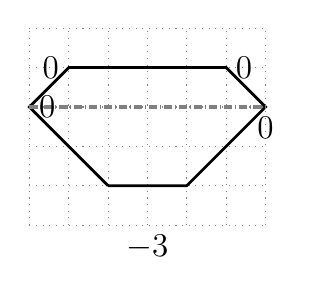
\begin{tikzpicture}[scale=0.5]
 	   \draw[dotted,step=1,gray] (-3,-3) grid (3,2); \draw[line width = 1pt] (-1,-2) --
     (-3,0) -- (-2,1)--(2,1)--
 	 (3,0)--(1,-2) -- (-1,-2); \draw[densely dashdotted, gray,line width = 1.2pt] (-3,0) -- (3,0);
 	 \node at (0,-3) [below] {\large{$-3$}};
 	 \node at (-3,0) [right] {\large{$0$}};
 	 \node at (-2,1) [left] {\large{$0$}};
 	 \node at (2,1) [right] {\large{$0$}};
 	 \node at (3,0) [below] {\large{$0$}};
	\end{tikzpicture}
	\caption*{$\Phi_1$}
\end{subfigure}
\begin{subfigure}[b]{0.30\textwidth}
	\centering
 	 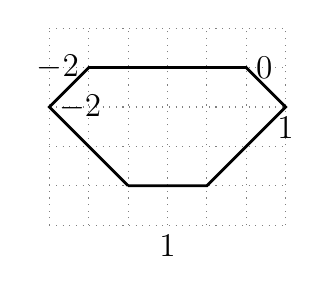
\begin{tikzpicture}[scale=0.5]
 	   \draw[dotted,step=1,gray] (-3,-3) grid (3,2); \draw[line width = 1pt] (-1,-2) --
     (-3,0) -- (-2,1)--(2,1)--
 	 (3,0)--(1,-2) -- (-1,-2);
 	 \node at (0,-3) [below] {\large{$1$}};
 	 \node at (-3,0) [right] {\large{$-2$}};
 	 \node at (-2,1) [left] {\large{$-2$}};
 	 \node at (2,1) [right] {\large{$0$}};
 	 \node at (3,0) [below] {\large{$1$}};
	\end{tikzpicture}
	\caption*{$\Phi_\infty$}
\end{subfigure}
\begin{subfigure}[b]{0.40\textwidth}
	\centering
 	 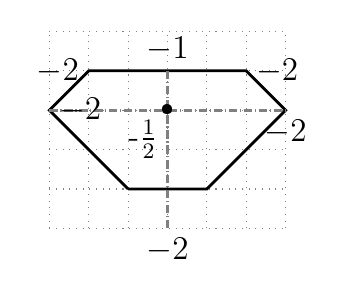
\begin{tikzpicture}[scale=0.5]
 	   \draw[dotted,step=1,gray] (-3,-3) grid (3,2); \draw[line width = 1pt] (-1,-2) --
     (-3,0) -- (-2,1)--(2,1)--
 	 (3,0)--(1,-2) -- (-1,-2); \draw[densely dashdotted, gray,line width = 1.2pt] (-3,0) -- (3,0); \draw[densely dashdotted, gray,line width = 1.2pt] (0,-3) -- (0,1) ;
 	 \node at (0,-3) [below] {\large{$-2$}};
 	 \node at (-3,0) [right] {\large{$-2$}};
 	 \node at (-2,1) [left] {\large{$-2$}};
 	 \node at (2,1) [right] {\large{$-2$}};
 	 \node at (3,0) [below] {\large{$-2$}};
 	 \node at (0,0) [below left] {\large{-$\frac{1}{2}$}};
 	 \node at (0,1) [above] {\large{$-1$}};
 	 \draw (0,0) node {\textbullet};
	\end{tikzpicture}
	\caption*{$\deg \Phi $}
\end{subfigure}
}
\end{figure}

\begin{align*}
g(\xi) &= \frac{1}{\xi_{2}^{4}}\cdot\left({\left(2 \, \xi_{2}^{3} - 3 \, \xi_{2} - 3\right)} e^{\left(4 \, \xi_{2}\right)} + 12 \, \xi_{2} e^{\left(3 \, \xi_{2}\right)} + 3 \, \xi_{2} + 3\right) e^{\left(-3 \, \xi_{2}\right)} \\
h_0(\xi_2) &= \frac{1}{3\xi_2^{4}}\cdot
{\left({\left(2   \xi_2^{3} - 3   \xi_2 - 3\right)} e^{4   \xi_2} + 3   {\left(3   \xi_2^{2} + 2\right)} e^{3   \xi_2} - 3   \xi_2 - 3\right)} e^{-3   \xi_2}
\\
h_1(\xi_2) &= \frac{1}{6   \xi_2^{4}}\cdot
{\left({\left(8   \xi_2^{3} + 6   \xi_2^{2} - 3\right)} e^{4   \xi_2} - 12   {\left(3   \xi_2^{2} - 3   \xi_2 + 1\right)} e^{3   \xi_2} + 12   \xi_2 + 15\right)} e^{-3   \xi_2} \\
h_\infty(\xi_2) &= -\frac{1}{6   \xi_2^{4}}\cdot
{\left(2   {\left(2   \xi_2^{3} - 3   \xi_2 - 3\right)} e^{4   \xi_2} - 3   {\left(3   \xi_2^{2} - 12   \xi_2 + 2\right)} e^{3   \xi_2} + 12   \xi_2 + 12\right)} e^{-3   \xi_2} \\
h_y(\xi_2) &= \frac{1}{6   \xi_2^{4}}\cdot{\left({\left(8   \xi_2^{3} + 6   \xi_2^{2} - 3\right)} e^{4   \xi_2 } - 3   {\left(3   \xi_2^{2} - 2\right)} e^{3   \xi_2} - 6   y - 3\right)} e^{-3   \xi_2} 
\end{align*}
\begin{align*}
1.087 &< h_0(\xi_2) < 1.458 \\
2.178 &< h_1(\xi_2) < 2.470 \\
0.446 &< h_\infty(\xi_2) < 0.827 \\
4.151 &< h_y(\xi_2) < 4.309 \ \ \ \ \ \ \   \left( \text{for } y \not \in \{0,1,\infty\} \right)
\end{align*}



\begin{tabular}{llll}
\toprule
\textbf{Name:} & 3.21 \hspace{0.3\textwidth} & \textbf{Description:} & Blow up of $Q$ in a line\\
\midrule
\end{tabular}

\begin{figure}[h]
\centering
\label{fig:data321}
\resizebox{0.9\linewidth}{!}{
\begin{subfigure}[b]{0.30\textwidth}
\centering
  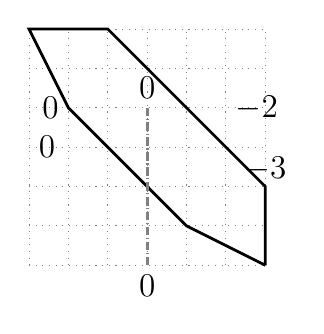
\begin{tikzpicture}[scale=0.5]
   	 \draw[dotted,step=1,gray,] (-3,-3) grid (3,3); \draw[line width = 1pt] (3,-3) --
     (1,-2) -- (-2,1)--(-3,3)--
 	 (-1,3)--(3,-1) -- (3,-3); \draw[densely dashdotted, gray, line width = 1.2pt] (0,-3) -- (0,1);
 	 \node at (0,-3) [below] {\large{$0$}};
 	 \node at (-3,0) [right] {\large{$0$}};
 	 \node at (-2,1) [left] {\large{$0$}};
 	 \node at (2,1) [right] {\large{$-2$}};
 	 \node at (3,0) [below] {\large{$-3$}};
 	 \node at (0,1) [above] {\large{$0$}};
	\end{tikzpicture}
	\caption*{$\Phi_0$}
\end{subfigure}
\begin{subfigure}[b]{0.30\textwidth}
	\centering
 	 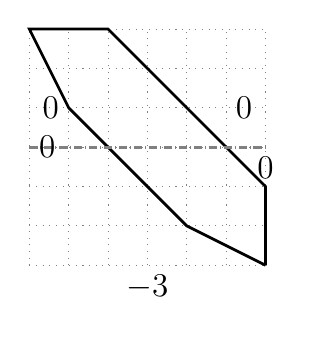
\begin{tikzpicture}[scale=0.5]
   	 \draw[dotted,step=1,gray,] (-3,-3) grid (3,3); \draw[line width = 1pt] (3,-3) --
     (1,-2) -- (-2,1)--(-3,3)--
 	 (-1,3)--(3,-1) -- (3,-3); \draw[densely dashdotted, gray,line width = 1.2pt] (-3,0) -- (3,0);
 	 \node at (0,-3) [below] {\large{$-3$}};
 	 \node at (-3,0) [right] {\large{$0$}};
 	 \node at (-2,1) [left] {\large{$0$}};
 	 \node at (2,1) [right] {\large{$0$}};
 	 \node at (3,0) [below] {\large{$0$}};
	\end{tikzpicture}
	\caption*{$\Phi_1$}
\end{subfigure}
\begin{subfigure}[b]{0.30\textwidth}
	\centering
 	 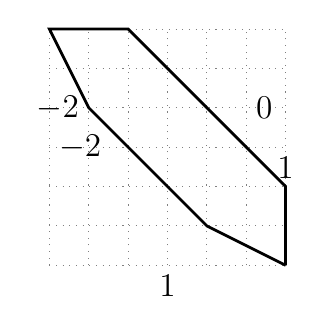
\begin{tikzpicture}[scale=0.5]
   	 \draw[dotted,step=1,gray,] (-3,-3) grid (3,3); \draw[line width = 1pt] (3,-3) --
     (1,-2) -- (-2,1)--(-3,3)--
 	 (-1,3)--(3,-1) -- (3,-3);
 	 \node at (0,-3) [below] {\large{$1$}};
 	 \node at (-3,0) [right] {\large{$-2$}};
 	 \node at (-2,1) [left] {\large{$-2$}};
 	 \node at (2,1) [right] {\large{$0$}};
 	 \node at (3,0) [below] {\large{$1$}};
	\end{tikzpicture}
	\caption*{$\Phi_\infty$}
\end{subfigure}
\begin{subfigure}[b]{0.40\textwidth}
	\centering
 	 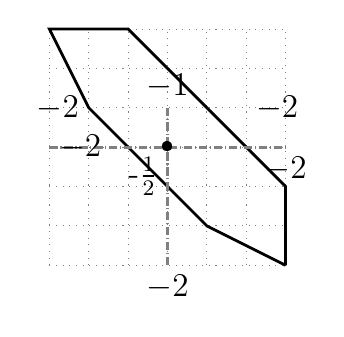
\begin{tikzpicture}[scale=0.5]
   	 \draw[dotted,step=1,gray,] (-3,-3) grid (3,3); \draw[line width = 1pt] (3,-3) --
     (1,-2) -- (-2,1)--(-3,3)--
 	 (-1,3)--(3,-1) -- (3,-3); \draw[densely dashdotted, gray,line width = 1.2pt] (-3,0) -- (3,0); \draw[densely dashdotted, gray,line width = 1.2pt] (0,-3) -- (0,1) ;
 	 \node at (0,-3) [below] {\large{$-2$}};
 	 \node at (-3,0) [right] {\large{$-2$}};
 	 \node at (-2,1) [left] {\large{$-2$}};
 	 \node at (2,1) [right] {\large{$-2$}};
 	 \node at (3,0) [below] {\large{$-2$}};
 	 \node at (0,0) [below left] {\large{-$\frac{1}{2}$}};
 	 \node at (0,1) [above] {\large{$-1$}};
 	 \draw (0,0) node {\textbullet};
	\end{tikzpicture}
	\caption*{$\deg \Phi $}
\end{subfigure}
}
\end{figure}

\begin{align*}
g(\xi) &= \frac{1}{\xi_{2}^{4}}\cdot\left({\left(2 \, \xi_{2}^{3} - 3 \, \xi_{2} - 3\right)} e^{\left(4 \, \xi_{2}\right)} + 12 \, \xi_{2} e^{\left(3 \, \xi_{2}\right)} + 3 \, \xi_{2} + 3\right) e^{\left(-3 \, \xi_{2}\right)} \\
h_0(\xi_2) &= \frac{1}{3\xi_2^{4}}\cdot
{\left({\left(2   \xi_2^{3} - 3   \xi_2 - 3\right)} e^{4   \xi_2} + 3   {\left(3   \xi_2^{2} + 2\right)} e^{3   \xi_2} - 3   \xi_2 - 3\right)} e^{-3   \xi_2}
\\
h_1(\xi_2) &= \frac{1}{6   \xi_2^{4}}\cdot
{\left({\left(8   \xi_2^{3} + 6   \xi_2^{2} - 3\right)} e^{4   \xi_2} - 12   {\left(3   \xi_2^{2} - 3   \xi_2 + 1\right)} e^{3   \xi_2} + 12   \xi_2 + 15\right)} e^{-3   \xi_2} \\
h_\infty(\xi_2) &= -\frac{1}{6   \xi_2^{4}}\cdot
{\left(2   {\left(2   \xi_2^{3} - 3   \xi_2 - 3\right)} e^{4   \xi_2} - 3   {\left(3   \xi_2^{2} - 12   \xi_2 + 2\right)} e^{3   \xi_2} + 12   \xi_2 + 12\right)} e^{-3   \xi_2} \\
h_y(\xi_2) &= \frac{1}{6   \xi_2^{4}}\cdot{\left({\left(8   \xi_2^{3} + 6   \xi_2^{2} - 3\right)} e^{4   \xi_2 } - 3   {\left(3   \xi_2^{2} - 2\right)} e^{3   \xi_2} - 6   y - 3\right)} e^{-3   \xi_2} 
\end{align*}
\begin{align*}
1.087 &< h_0(\xi_2) < 1.458 \\
2.178 &< h_1(\xi_2) < 2.470 \\
0.446 &< h_\infty(\xi_2) < 0.827 \\
4.151 &< h_y(\xi_2) < 4.309 \ \ \ \ \ \ \   \left( \text{for } y \not \in \{0,1,\infty\} \right)
\end{align*}


\begin{tabular}{llll}
\toprule
\textbf{Name:} & 3.22 \hspace{0.3\textwidth} & \textbf{Description:} & Blow up of $Q$ in a line\\
\midrule
\end{tabular}

\begin{figure}[h]
\centering

\label{fig:data322}
\resizebox{0.9\linewidth}{!}{
\begin{subfigure}[b]{0.30\textwidth}
\centering
  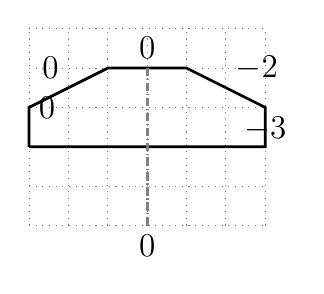
\begin{tikzpicture}[scale=0.5]
   	 \draw[dotted,step=1,gray,] (-3,-3) grid (3,2); \draw[line width = 1pt] (-3,-1) --
     (-3,0) -- (-1,1)--(1,1)--
 	 (3,0)--(3,-1) -- (-3,-1); \draw[densely dashdotted, gray, line width = 1.2pt] (0,-3) -- (0,1);
 	 \node at (0,-3) [below] {\large{$0$}};
 	 \node at (-3,0) [right] {\large{$0$}};
 	 \node at (-2,1) [left] {\large{$0$}};
 	 \node at (2,1) [right] {\large{$-2$}};
 	 \node at (3,0) [below] {\large{$-3$}};
 	 \node at (0,1) [above] {\large{$0$}};
	\end{tikzpicture}
	\caption*{$\Phi_0$}
\end{subfigure}
\begin{subfigure}[b]{0.30\textwidth}
	\centering
 	 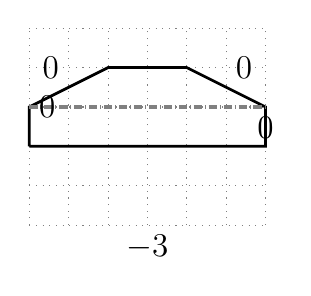
\begin{tikzpicture}[scale=0.5]
 	   \draw[dotted,step=1,gray] (-3,-3) grid (3,2); \draw[line width = 1pt] (-3,-1) --
     (-3,0) -- (-1,1)--(1,1)--
 	 (3,0)--(3,-1) -- (-3,-1); \draw[densely dashdotted, gray,line width = 1.2pt] (-3,0) -- (3,0);
 	 \node at (0,-3) [below] {\large{$-3$}};
 	 \node at (-3,0) [right] {\large{$0$}};
 	 \node at (-2,1) [left] {\large{$0$}};
 	 \node at (2,1) [right] {\large{$0$}};
 	 \node at (3,0) [below] {\large{$0$}};
	\end{tikzpicture}
	\caption*{$\Phi_1$}
\end{subfigure}
\begin{subfigure}[b]{0.30\textwidth}
	\centering
 	 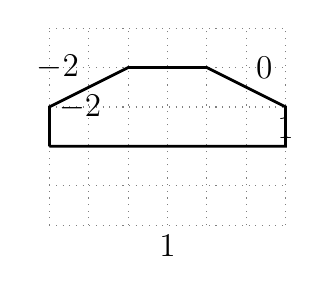
\begin{tikzpicture}[scale=0.5]
 	   \draw[dotted,step=1,gray] (-3,-3) grid (3,2); \draw[line width = 1pt] (-3,-1) --
     (-3,0) -- (-1,1)--(1,1)--
 	 (3,0)--(3,-1) -- (-3,-1);
 	 \node at (0,-3) [below] {\large{$1$}};
 	 \node at (-3,0) [right] {\large{$-2$}};
 	 \node at (-2,1) [left] {\large{$-2$}};
 	 \node at (2,1) [right] {\large{$0$}};
 	 \node at (3,0) [below] {\large{$1$}};
	\end{tikzpicture}
	\caption*{$\Phi_\infty$}
\end{subfigure}
\begin{subfigure}[b]{0.40\textwidth}
	\centering
 	 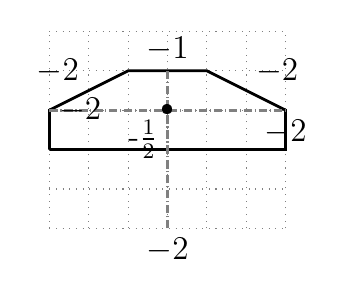
\begin{tikzpicture}[scale=0.5]
 	   \draw[dotted,step=1,gray] (-3,-3) grid (3,2); \draw[line width = 1pt] (-3,-1) --
     (-3,0) -- (-1,1)--(1,1)--
 	 (3,0)--(3,-1) -- (-3,-1); \draw[densely dashdotted, gray,line width = 1.2pt] (-3,0) -- (3,0); \draw[densely dashdotted, gray,line width = 1.2pt] (0,-3) -- (0,1) ;
 	 \node at (0,-3) [below] {\large{$-2$}};
 	 \node at (-3,0) [right] {\large{$-2$}};
 	 \node at (-2,1) [left] {\large{$-2$}};
 	 \node at (2,1) [right] {\large{$-2$}};
 	 \node at (3,0) [below] {\large{$-2$}};
 	 \node at (0,0) [below left] {\large{-$\frac{1}{2}$}};
 	 \node at (0,1) [above] {\large{$-1$}};
 	 \draw (0,0) node {\textbullet};
	\end{tikzpicture}
	\caption*{$\deg \Phi $}
\end{subfigure}
}
\end{figure}

\begin{align*}
g(\xi) &= \frac{1}{\xi_{2}^{4}}\cdot\left({\left(2 \, \xi_{2}^{3} - 3 \, \xi_{2} - 3\right)} e^{\left(4 \, \xi_{2}\right)} + 12 \, \xi_{2} e^{\left(3 \, \xi_{2}\right)} + 3 \, \xi_{2} + 3\right) e^{\left(-3 \, \xi_{2}\right)} \\
h_0(\xi_2) &= \frac{1}{3\xi_2^{4}}\cdot
{\left({\left(2   \xi_2^{3} - 3   \xi_2 - 3\right)} e^{4   \xi_2} + 3   {\left(3   \xi_2^{2} + 2\right)} e^{3   \xi_2} - 3   \xi_2 - 3\right)} e^{-3   \xi_2}
\\
h_1(\xi_2) &= \frac{1}{6   \xi_2^{4}}\cdot
{\left({\left(8   \xi_2^{3} + 6   \xi_2^{2} - 3\right)} e^{4   \xi_2} - 12   {\left(3   \xi_2^{2} - 3   \xi_2 + 1\right)} e^{3   \xi_2} + 12   \xi_2 + 15\right)} e^{-3   \xi_2} \\
h_\infty(\xi_2) &= -\frac{1}{6   \xi_2^{4}}\cdot
{\left(2   {\left(2   \xi_2^{3} - 3   \xi_2 - 3\right)} e^{4   \xi_2} - 3   {\left(3   \xi_2^{2} - 12   \xi_2 + 2\right)} e^{3   \xi_2} + 12   \xi_2 + 12\right)} e^{-3   \xi_2} \\
h_y(\xi_2) &= \frac{1}{6   \xi_2^{4}}\cdot{\left({\left(8   \xi_2^{3} + 6   \xi_2^{2} - 3\right)} e^{4   \xi_2 } - 3   {\left(3   \xi_2^{2} - 2\right)} e^{3   \xi_2} - 6   y - 3\right)} e^{-3   \xi_2} 
\end{align*}
\begin{align*}
1.087 &< h_0(\xi_2) < 1.458 \\
2.178 &< h_1(\xi_2) < 2.470 \\
0.446 &< h_\infty(\xi_2) < 0.827 \\
4.151 &< h_y(\xi_2) < 4.309 \ \ \ \ \ \ \   \left( \text{for } y \not \in \{0,1,\infty\} \right)
\end{align*}




\begin{tabular}{llll}
\toprule
\textbf{Name:} & 3.23 \hspace{0.3\textwidth} & \textbf{Description:} & Blow up of $Q$ in a line\\
\midrule
\end{tabular}

\begin{figure}[h]
\centering
\label{fig:data323}
\resizebox{0.9\linewidth}{!}{
\begin{subfigure}[b]{0.30\textwidth}
\centering
  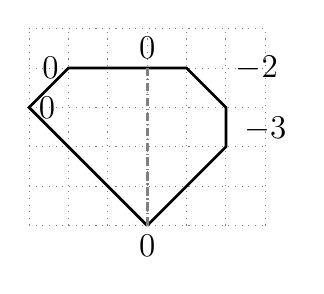
\begin{tikzpicture}[scale=0.5]
   	 \draw[dotted,step=1,gray,] (-3,-3) grid (3,2); \draw[line width = 1pt] (0,-3) --
     (-3,0) -- (-2,1)--(1,1)--
 	 (2,0)--(2,-1) -- (0,-3); \draw[densely dashdotted, gray, line width = 1.2pt] (0,-3) -- (0,1);
 	 \node at (0,-3) [below] {\large{$0$}};
 	 \node at (-3,0) [right] {\large{$0$}};
 	 \node at (-2,1) [left] {\large{$0$}};
 	 \node at (2,1) [right] {\large{$-2$}};
 	 \node at (3,0) [below] {\large{$-3$}};
 	 \node at (0,1) [above] {\large{$0$}};
	\end{tikzpicture}
	\caption*{$\Phi_0$}
\end{subfigure}
\begin{subfigure}[b]{0.30\textwidth}
	\centering
 	 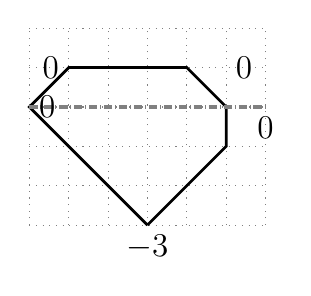
\begin{tikzpicture}[scale=0.5]
 	   \draw[dotted,step=1,gray] (-3,-3) grid (3,2); \draw[line width = 1pt] (0,-3) --
     (-3,0) -- (-2,1)--(1,1)--
 	 (2,0)--(2,-1) -- (0,-3); \draw[densely dashdotted, gray,line width = 1.2pt] (-3,0) -- (3,0);
 	 \node at (0,-3) [below] {\large{$-3$}};
 	 \node at (-3,0) [right] {\large{$0$}};
 	 \node at (-2,1) [left] {\large{$0$}};
 	 \node at (2,1) [right] {\large{$0$}};
 	 \node at (3,0) [below] {\large{$0$}};
	\end{tikzpicture}
	\caption*{$\Phi_1$}
\end{subfigure}
\begin{subfigure}[b]{0.30\textwidth}
	\centering
 	 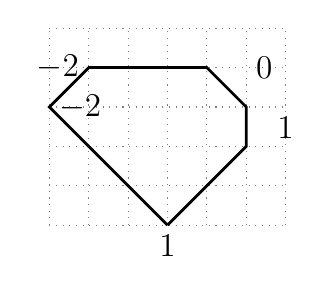
\begin{tikzpicture}[scale=0.5]
 	   \draw[dotted,step=1,gray] (-3,-3) grid (3,2); \draw[line width = 1pt] (0,-3) --
     (-3,0) -- (-2,1)--(1,1)--
 	 (2,0)--(2,-1) -- (0,-3);
 	 \node at (0,-3) [below] {\large{$1$}};
 	 \node at (-3,0) [right] {\large{$-2$}};
 	 \node at (-2,1) [left] {\large{$-2$}};
 	 \node at (2,1) [right] {\large{$0$}};
 	 \node at (3,0) [below] {\large{$1$}};
	\end{tikzpicture}
	\caption*{$\Phi_\infty$}
\end{subfigure}
\begin{subfigure}[b]{0.40\textwidth}
	\centering
 	 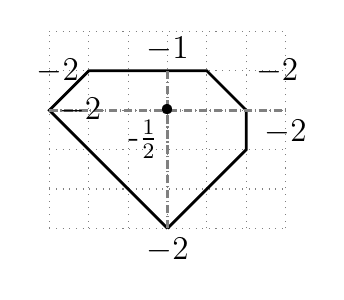
\begin{tikzpicture}[scale=0.5]
 	   \draw[dotted,step=1,gray] (-3,-3) grid (3,2); \draw[line width = 1pt] (0,-3) --
     (-3,0) -- (-2,1)--(1,1)--
 	 (2,0)--(2,-1) -- (0,-3); \draw[densely dashdotted, gray,line width = 1.2pt] (-3,0) -- (3,0); \draw[densely dashdotted, gray,line width = 1.2pt] (0,-3) -- (0,1) ;
 	 \node at (0,-3) [below] {\large{$-2$}};
 	 \node at (-3,0) [right] {\large{$-2$}};
 	 \node at (-2,1) [left] {\large{$-2$}};
 	 \node at (2,1) [right] {\large{$-2$}};
 	 \node at (3,0) [below] {\large{$-2$}};
 	 \node at (0,0) [below left] {\large{-$\frac{1}{2}$}};
 	 \node at (0,1) [above] {\large{$-1$}};
 	 \draw (0,0) node {\textbullet};
	\end{tikzpicture}
	\caption*{$\deg \Phi $}
\end{subfigure}
}
\end{figure}

\begin{align*}
g(\xi) &= \frac{1}{\xi_{2}^{4}}\cdot\left({\left(2 \, \xi_{2}^{3} - 3 \, \xi_{2} - 3\right)} e^{\left(4 \, \xi_{2}\right)} + 12 \, \xi_{2} e^{\left(3 \, \xi_{2}\right)} + 3 \, \xi_{2} + 3\right) e^{\left(-3 \, \xi_{2}\right)} \\
h_0(\xi_2) &= \frac{1}{3\xi_2^{4}}\cdot
{\left({\left(2   \xi_2^{3} - 3   \xi_2 - 3\right)} e^{4   \xi_2} + 3   {\left(3   \xi_2^{2} + 2\right)} e^{3   \xi_2} - 3   \xi_2 - 3\right)} e^{-3   \xi_2}
\\
h_1(\xi_2) &= \frac{1}{6   \xi_2^{4}}\cdot
{\left({\left(8   \xi_2^{3} + 6   \xi_2^{2} - 3\right)} e^{4   \xi_2} - 12   {\left(3   \xi_2^{2} - 3   \xi_2 + 1\right)} e^{3   \xi_2} + 12   \xi_2 + 15\right)} e^{-3   \xi_2} \\
h_\infty(\xi_2) &= -\frac{1}{6   \xi_2^{4}}\cdot
{\left(2   {\left(2   \xi_2^{3} - 3   \xi_2 - 3\right)} e^{4   \xi_2} - 3   {\left(3   \xi_2^{2} - 12   \xi_2 + 2\right)} e^{3   \xi_2} + 12   \xi_2 + 12\right)} e^{-3   \xi_2} \\
h_y(\xi_2) &= \frac{1}{6   \xi_2^{4}}\cdot{\left({\left(8   \xi_2^{3} + 6   \xi_2^{2} - 3\right)} e^{4   \xi_2 } - 3   {\left(3   \xi_2^{2} - 2\right)} e^{3   \xi_2} - 6   y - 3\right)} e^{-3   \xi_2} 
\end{align*}
\begin{align*}
1.087 &< h_0(\xi_2) < 1.458 \\
2.178 &< h_1(\xi_2) < 2.470 \\
0.446 &< h_\infty(\xi_2) < 0.827 \\
4.151 &< h_y(\xi_2) < 4.309 \ \ \ \ \ \ \   \left( \text{for } y \not \in \{0,1,\infty\} \right)
\end{align*}


\begin{tabular}{llll}
\toprule
\textbf{Name:} & 3.24 \hspace{0.3\textwidth} & \textbf{Description:} & Blow up of $Q$ in a line\\
\midrule
\end{tabular}

\begin{figure}[h]
\centering


\label{fig:data324}
\resizebox{0.9\linewidth}{!}{
\begin{subfigure}[b]{0.30\textwidth}
\centering
  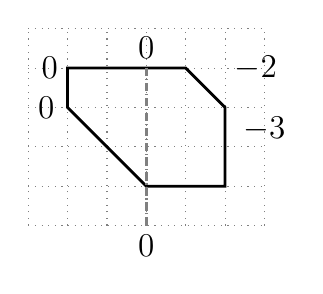
\begin{tikzpicture}[scale=0.5]
   	 \draw[dotted,step=1,gray,] (-3,-3) grid (3,2); \draw[line width = 1pt] (0,-2) --
     (-2,0) -- (-2,1)--(1,1)--
 	 (2,0)--(2,-2) -- (0,-2); \draw[densely dashdotted, gray, line width = 1.2pt] (0,-3) -- (0,1);
 	 \node at (0,-3) [below] {\large{$0$}};
 	 \node at (-3,0) [right] {\large{$0$}};
 	 \node at (-2,1) [left] {\large{$0$}};
 	 \node at (2,1) [right] {\large{$-2$}};
 	 \node at (3,0) [below] {\large{$-3$}};
 	 \node at (0,1) [above] {\large{$0$}};
	\end{tikzpicture}
	\caption*{$\Phi_0$}
\end{subfigure}
\begin{subfigure}[b]{0.30\textwidth}
	\centering
 	 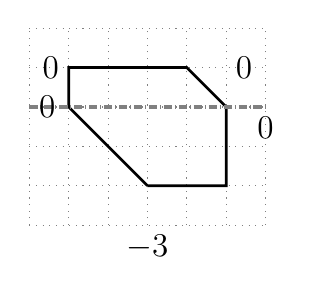
\begin{tikzpicture}[scale=0.5]
 	   \draw[dotted,step=1,gray] (-3,-3) grid (3,2); \draw[line width = 1pt] (0,-2) --
     (-2,0) -- (-2,1)--(1,1)--
 	 (2,0)--(2,-2) -- (0,-2); \draw[densely dashdotted, gray,line width = 1.2pt] (-3,0) -- (3,0);
 	 \node at (0,-3) [below] {\large{$-3$}};
 	 \node at (-3,0) [right] {\large{$0$}};
 	 \node at (-2,1) [left] {\large{$0$}};
 	 \node at (2,1) [right] {\large{$0$}};
 	 \node at (3,0) [below] {\large{$0$}};
	\end{tikzpicture}
	\caption*{$\Phi_1$}
\end{subfigure}
\begin{subfigure}[b]{0.30\textwidth}
	\centering
 	 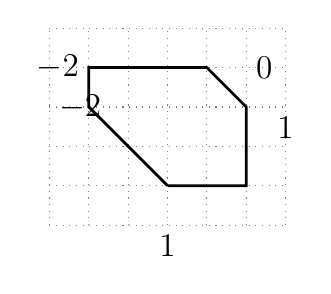
\begin{tikzpicture}[scale=0.5]
 	   \draw[dotted,step=1,gray] (-3,-3) grid (3,2); \draw[line width = 1pt] (0,-2) --
     (-2,0) -- (-2,1)--(1,1)--
 	 (2,0)--(2,-2) -- (0,-2);
 	 \node at (0,-3) [below] {\large{$1$}};
 	 \node at (-3,0) [right] {\large{$-2$}};
 	 \node at (-2,1) [left] {\large{$-2$}};
 	 \node at (2,1) [right] {\large{$0$}};
 	 \node at (3,0) [below] {\large{$1$}};
	\end{tikzpicture}
	\caption*{$\Phi_\infty$}
\end{subfigure}
\begin{subfigure}[b]{0.40\textwidth}
	\centering
 	 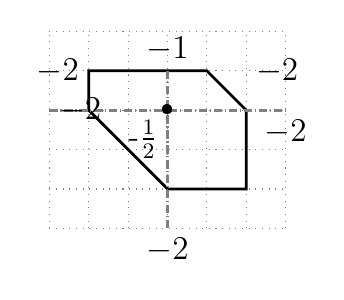
\begin{tikzpicture}[scale=0.5]
 	   \draw[dotted,step=1,gray] (-3,-3) grid (3,2); \draw[line width = 1pt] (0,-2) --
     (-2,0) -- (-2,1)--(1,1)--
 	 (2,0)--(2,-2) -- (0,-2); \draw[densely dashdotted, gray,line width = 1.2pt] (-3,0) -- (3,0); \draw[densely dashdotted, gray,line width = 1.2pt] (0,-3) -- (0,1) ;
 	 \node at (0,-3) [below] {\large{$-2$}};
 	 \node at (-3,0) [right] {\large{$-2$}};
 	 \node at (-2,1) [left] {\large{$-2$}};
 	 \node at (2,1) [right] {\large{$-2$}};
 	 \node at (3,0) [below] {\large{$-2$}};
 	 \node at (0,0) [below left] {\large{-$\frac{1}{2}$}};
 	 \node at (0,1) [above] {\large{$-1$}};
 	 \draw (0,0) node {\textbullet};
	\end{tikzpicture}
	\caption*{$\deg \Phi $}
\end{subfigure}
}
\end{figure}

\begin{align*}
g(\xi) &= \frac{1}{\xi_{2}^{4}}\cdot\left({\left(2 \, \xi_{2}^{3} - 3 \, \xi_{2} - 3\right)} e^{\left(4 \, \xi_{2}\right)} + 12 \, \xi_{2} e^{\left(3 \, \xi_{2}\right)} + 3 \, \xi_{2} + 3\right) e^{\left(-3 \, \xi_{2}\right)} \\
h_0(\xi_2) &= \frac{1}{3\xi_2^{4}}\cdot
{\left({\left(2   \xi_2^{3} - 3   \xi_2 - 3\right)} e^{4   \xi_2} + 3   {\left(3   \xi_2^{2} + 2\right)} e^{3   \xi_2} - 3   \xi_2 - 3\right)} e^{-3   \xi_2}
\\
h_1(\xi_2) &= \frac{1}{6   \xi_2^{4}}\cdot
{\left({\left(8   \xi_2^{3} + 6   \xi_2^{2} - 3\right)} e^{4   \xi_2} - 12   {\left(3   \xi_2^{2} - 3   \xi_2 + 1\right)} e^{3   \xi_2} + 12   \xi_2 + 15\right)} e^{-3   \xi_2} \\
h_\infty(\xi_2) &= -\frac{1}{6   \xi_2^{4}}\cdot
{\left(2   {\left(2   \xi_2^{3} - 3   \xi_2 - 3\right)} e^{4   \xi_2} - 3   {\left(3   \xi_2^{2} - 12   \xi_2 + 2\right)} e^{3   \xi_2} + 12   \xi_2 + 12\right)} e^{-3   \xi_2} \\
h_y(\xi_2) &= \frac{1}{6   \xi_2^{4}}\cdot{\left({\left(8   \xi_2^{3} + 6   \xi_2^{2} - 3\right)} e^{4   \xi_2 } - 3   {\left(3   \xi_2^{2} - 2\right)} e^{3   \xi_2} - 6   y - 3\right)} e^{-3   \xi_2} 
\end{align*}
\begin{align*}
1.087 &< h_0(\xi_2) < 1.458 \\
2.178 &< h_1(\xi_2) < 2.470 \\
0.446 &< h_\infty(\xi_2) < 0.827 \\
4.151 &< h_y(\xi_2) < 4.309 \ \ \ \ \ \ \   \left( \text{for } y \not \in \{0,1,\infty\} \right)
\end{align*}



\begin{tabular}{llll}
\toprule
\textbf{Name:} & 4.5* \hspace{0.3\textwidth} & \textbf{Description:} & Blow up of $Q$ in a line\\
\midrule
\end{tabular}

%\begin{figure}[h]
%\centering
%
%\label{fig:data45*}
%\resizebox{0.9\linewidth}{!}{
%\begin{subfigure}[b]{0.30\textwidth}
%\centering
%  \begin{tikzpicture}[scale=0.5]
%   	 \draw[dotted,step=1,gray,] (-3,-3) grid (3,3); \draw[line width = 1pt] (3,-3) --
%     (1,-2) -- (-2,1)--(-3,3)--
% 	 (-2,3)--(3,-2) -- (3,-3); \draw[densely dashdotted, gray, line width = 1.2pt] (0,-3) -- (0,1);
% 	 \node at (3,-3) [below] {\large{$-2$}};
% 	 \node at (1,-2) [right] {\large{$0$}};
% 	 \node at (-2,1) [left] {\large{$0$}};
% 	 \node at (-3,3) [right] {\large{$0$}};
% 	 \node at (-2,3) [right] {\large{$-2$}};
% 	 \node at (3,-2) [right] {\large{$-2$}};
%	\end{tikzpicture}
%	\caption*{$\Phi_0$}
%\end{subfigure}
%\begin{subfigure}[b]{0.30\textwidth}
%	\centering
% 	 \begin{tikzpicture}[scale=0.5]
% 	   \draw[dotted,step=1,gray] (-3,-3) grid (3,3); \draw[line width = 1pt] (3,-3) --
%     (1,-2) -- (-2,1)--(-3,3)--
% 	 (-2,3)--(3,-2) -- (3,-3); \draw[densely dashdotted, gray,line width = 1.2pt] (-3,0) -- (3,0);
% 	 \node at (3,-3) [below] {\large{$-2$}};
% 	 \node at (1,-2) [right] {\large{$0$}};
% 	 \node at (-2,1) [left] {\large{$0$}};
% 	 \node at (-3,3) [right] {\large{$0$}};
% 	 \node at (-2,3) [right] {\large{$-2$}};
% 	 \node at (3,-2) [right] {\large{$-2$}};
%	\end{tikzpicture}
%	\caption*{$\Phi_1$}
%\end{subfigure}
%\begin{subfigure}[b]{0.30\textwidth}
%	\centering
% 	 \begin{tikzpicture}[scale=0.5]
% 	   \draw[dotted,step=1,gray] (-3,-3) grid (3,3); \draw[line width = 1pt] (3,-3) --
%     (1,-2) -- (-2,1)--(-3,3)--
% 	 (-2,3)--(3,-2) -- (3,-3);
% 	 \node at (3,-3) [below] {\large{$-2$}};
% 	 \node at (1,-2) [right] {\large{$0$}};
% 	 \node at (-2,1) [left] {\large{$0$}};
% 	 \node at (-3,3) [right] {\large{$0$}};
% 	 \node at (-2,3) [right] {\large{$-2$}};
% 	 \node at (3,-2) [right] {\large{$-2$}};
%	\end{tikzpicture}
%	\caption*{$\Phi_\infty$}
%\end{subfigure}
%\begin{subfigure}[b]{0.40\textwidth}
%	\centering
% 	 \begin{tikzpicture}[scale=0.5]
% 	   \draw[dotted,step=1,gray] (-3,-3) grid (3,3); \draw[line width = 1pt] (3,-3) --
%     (1,-2) -- (-2,1)--(-3,3)--
% 	 (-2,3)--(3,-2) -- (3,-3); \draw[densely dashdotted, gray,line width = 1.2pt] (0,-1) -- (2,-1); \draw[densely dashdotted, gray,line width = 1.2pt] (-1,0) -- (-1,2) ; \draw[densely dashdotted, gray,line width = 1.2pt] (3,-3) -- (-3,3)
% 	 \node at (3,-3) [right] {\large{$-2$}};
% 	 \node at (1,-2) [below] {\large{$0$}};
% 	 \node at (-2,1) [left] {\large{$0$}};
% 	 \node at (-3,3) [left] {\large{$0$}};
% 	 \node at (-2,3) [above] {\large{$-2$}};
% 	 \node at (3,-2) [right] {\large{$-2$}};
% 	 \node at (2,-1) [right] {\large{$-\frac{3}{2}$}};
% 	 \node at (0,-1) [below left] {\large{$-\frac{3}{2}$}};
% 	 \node at (-1,2) [above] {\large{$-\frac{3}{2}$}};
% 	 \node at (-1,0) [left] {\large{$-\frac{3}{2}$}};
% 	 \draw (0,0) node {\textbullet};
%	\end{tikzpicture}
%	\caption*{$\deg \Phi $}
%\end{subfigure}
%}
%\end{figure}

\begin{align*}
g(\xi) &= \frac{1}{\xi_{2}^{4}}\cdot\left({\left(2 \, \xi_{2}^{3} - 3 \, \xi_{2} - 3\right)} e^{\left(4 \, \xi_{2}\right)} + 12 \, \xi_{2} e^{\left(3 \, \xi_{2}\right)} + 3 \, \xi_{2} + 3\right) e^{\left(-3 \, \xi_{2}\right)} \\
h_0(\xi_2) &= \frac{1}{3\xi_2^{4}}\cdot
{\left({\left(2   \xi_2^{3} - 3   \xi_2 - 3\right)} e^{4   \xi_2} + 3   {\left(3   \xi_2^{2} + 2\right)} e^{3   \xi_2} - 3   \xi_2 - 3\right)} e^{-3   \xi_2}
\\
h_1(\xi_2) &= \frac{1}{6   \xi_2^{4}}\cdot
{\left({\left(8   \xi_2^{3} + 6   \xi_2^{2} - 3\right)} e^{4   \xi_2} - 12   {\left(3   \xi_2^{2} - 3   \xi_2 + 1\right)} e^{3   \xi_2} + 12   \xi_2 + 15\right)} e^{-3   \xi_2} \\
h_\infty(\xi_2) &= -\frac{1}{6   \xi_2^{4}}\cdot
{\left(2   {\left(2   \xi_2^{3} - 3   \xi_2 - 3\right)} e^{4   \xi_2} - 3   {\left(3   \xi_2^{2} - 12   \xi_2 + 2\right)} e^{3   \xi_2} + 12   \xi_2 + 12\right)} e^{-3   \xi_2} \\
h_y(\xi_2) &= \frac{1}{6   \xi_2^{4}}\cdot{\left({\left(8   \xi_2^{3} + 6   \xi_2^{2} - 3\right)} e^{4   \xi_2 } - 3   {\left(3   \xi_2^{2} - 2\right)} e^{3   \xi_2} - 6   y - 3\right)} e^{-3   \xi_2} 
\end{align*}
\begin{align*}
1.087 &< h_0(\xi_2) < 1.458 \\
2.178 &< h_1(\xi_2) < 2.470 \\
0.446 &< h_\infty(\xi_2) < 0.827 \\
4.151 &< h_y(\xi_2) < 4.309 \ \ \ \ \ \ \   \left( \text{for } y \not \in \{0,1,\infty\} \right)
\end{align*}


\begin{tabular}{llll}
\toprule
\textbf{Name:} & 4.8 \hspace{0.3\textwidth} & \textbf{Description:} & Blow up of $Q$ in a line\\
\midrule
\end{tabular}


\begin{figure}[h]
\centering


\label{fig:data48}
\resizebox{0.9\linewidth}{!}{
\begin{subfigure}[b]{0.30\textwidth}
\centering
  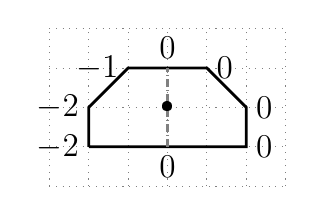
\begin{tikzpicture}[scale=0.5]
   	 \draw[dotted,step=1,gray,] (-3,-2) grid (3,2); \draw[line width = 1pt] (-2,-1) --
     (-2,0) -- (-1,1)--(1,1)--
 	 (2,0)--(2,-1) -- (-2,-1); \draw[densely dashdotted, gray, line width = 1.2pt] (0,-1) -- (0,1);
 	 \node at (-2,-1) [left] {\large{$-2$}};
 	 \node at (-2,0) [left] {\large{$-2$}};
 	 \node at (-1,1) [left] {\large{$-1$}};
 	 \node at (0,1) [above] {\large{$0$}};
 	 \node at (1,1) [right] {\large{$0$}};
 	 \node at (2,0) [right] {\large{$0$}};
 	 \node at (2,-1) [right] {\large{$0$}};
 	 \node at (0,-1) [below] {\large{$0$}};
 	 \draw (0,0) node {\textbullet};
	\end{tikzpicture}
	\caption*{$\Phi_0$}
\end{subfigure}
\begin{subfigure}[b]{0.30\textwidth}
	\centering
 	 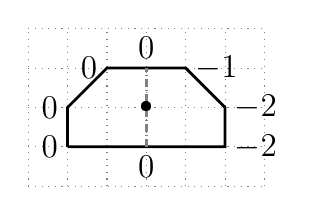
\begin{tikzpicture}[scale=0.5]
 	   \draw[dotted,step=1,gray] (-3,-2) grid (3,2); \draw[line width = 1pt] (-2,-1) --
     (-2,0) -- (-1,1)--(1,1)--
 	 (2,0)--(2,-1) -- (-2,-1); \draw[densely dashdotted, gray,line width = 1.2pt] (0,-1) -- (0,1); 
 	 \node at (-2,-1) [left] {\large{$0$}};
 	 \node at (-2,0) [left] {\large{$0$}};
 	 \node at (-1,1) [left] {\large{$0$}};
 	 \node at (0,1) [above] {\large{$0$}};
 	 \node at (1,1) [right] {\large{$-1$}};
 	 \node at (2,0) [right] {\large{$-2$}};
 	 \node at (2,-1) [right] {\large{$-2$}};
 	 \node at (0,-1) [below] {\large{$0$}};
 	 \draw (0,0) node {\textbullet};
	\end{tikzpicture}
	\caption*{$\Phi_1$}
\end{subfigure}
\begin{subfigure}[b]{0.30\textwidth}
	\centering
 	 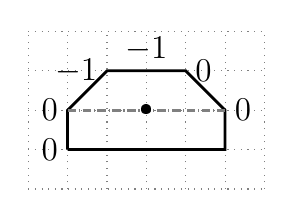
\begin{tikzpicture}[scale=0.5]
 	   \draw[dotted,step=1,gray] (-3,-2) grid (3,2); \draw[line width = 1pt] (-2,-1) --
     (-2,0) -- (-1,1)--(1,1)--
 	 (2,0)--(2,-1) -- (-2,-1); \draw[densely dashdotted, gray,line width = 1.2pt] (-2,0) -- (2,0) ;
 	 \node at (-2,-1) [left] {\large{$0$}};
 	 \node at (-2,0) [left] {\large{$0$}};
 	 \node at (-1,1) [left] {\large{$-1$}};
 	 \node at (0,1) [above] {\large{$-1$}};
 	 \node at (1,1) [right] {\large{$0$}};
 	 \node at (2,0) [right] {\large{$0$}};
 	 \draw (0,0) node {\textbullet};
	\end{tikzpicture}
	\caption*{$\Phi_\infty$}
\end{subfigure}
\begin{subfigure}[b]{0.40\textwidth}
	\centering
 	 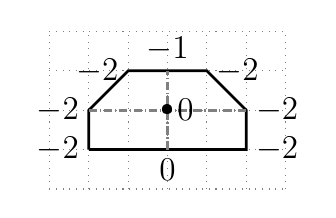
\begin{tikzpicture}[scale=0.5]
 	   \draw[dotted,step=1,gray] (-3,-2) grid (3,2); \draw[line width = 1pt] (-2,-1) --
     (-2,0) -- (-1,1)--(1,1)--
 	 (2,0)--(2,-1) -- (-2,-1); \draw[densely dashdotted, gray,line width = 1.2pt] (-2,0) -- (2,0); \draw[densely dashdotted, gray,line width = 1.2pt] (0,-1) -- (0,1) ;
 	 \node at (-2,-1) [left] {\large{$-2$}};
 	 \node at (-2,0) [left] {\large{$-2$}};
 	 \node at (-1,1) [left] {\large{$-2$}};
 	 \node at (0,1) [above] {\large{$-1$}};
 	 \node at (1,1) [right] {\large{$-2$}};
 	 \node at (2,0) [right] {\large{$-2$}};
 	 \node at (2,-1) [right] {\large{$-2$}};
 	 \node at (0,-1) [below] {\large{$0$}};
  	 \node at (0,0) [right] {\large{$0$}};
 	 \draw (0,0) node {\textbullet};
	\end{tikzpicture}
	\caption*{$\deg \Phi $}
\end{subfigure}
}
\end{figure}

\begin{align*}
g(\xi) &= \frac{1}{\xi_{2}^{4}}\cdot\left({\left(2 \, \xi_{2}^{3} - 3 \, \xi_{2} - 3\right)} e^{\left(4 \, \xi_{2}\right)} + 12 \, \xi_{2} e^{\left(3 \, \xi_{2}\right)} + 3 \, \xi_{2} + 3\right) e^{\left(-3 \, \xi_{2}\right)} \\
h_0(\xi_2) &= \frac{1}{3\xi_2^{4}}\cdot
{\left({\left(2   \xi_2^{3} - 3   \xi_2 - 3\right)} e^{4   \xi_2} + 3   {\left(3   \xi_2^{2} + 2\right)} e^{3   \xi_2} - 3   \xi_2 - 3\right)} e^{-3   \xi_2}
\\
h_1(\xi_2) &= \frac{1}{6   \xi_2^{4}}\cdot
{\left({\left(8   \xi_2^{3} + 6   \xi_2^{2} - 3\right)} e^{4   \xi_2} - 12   {\left(3   \xi_2^{2} - 3   \xi_2 + 1\right)} e^{3   \xi_2} + 12   \xi_2 + 15\right)} e^{-3   \xi_2} \\
h_\infty(\xi_2) &= -\frac{1}{6   \xi_2^{4}}\cdot
{\left(2   {\left(2   \xi_2^{3} - 3   \xi_2 - 3\right)} e^{4   \xi_2} - 3   {\left(3   \xi_2^{2} - 12   \xi_2 + 2\right)} e^{3   \xi_2} + 12   \xi_2 + 12\right)} e^{-3   \xi_2} \\
h_y(\xi_2) &= \frac{1}{6   \xi_2^{4}}\cdot{\left({\left(8   \xi_2^{3} + 6   \xi_2^{2} - 3\right)} e^{4   \xi_2 } - 3   {\left(3   \xi_2^{2} - 2\right)} e^{3   \xi_2} - 6   y - 3\right)} e^{-3   \xi_2} 
\end{align*}
\begin{align*}
1.087 &< h_0(\xi_2) < 1.458 \\
2.178 &< h_1(\xi_2) < 2.470 \\
0.446 &< h_\infty(\xi_2) < 0.827 \\
4.151 &< h_y(\xi_2) < 4.309 \ \ \ \ \ \ \   \left( \text{for } y \not \in \{0,1,\infty\} \right)
\end{align*}
